%%%%%%%%%%%%%%%%%%%%%%%%%%%%%%%%%%%%%%%%%%%%%%%%%%%%%%%%%%%%%%%%%%%%%%%%%%%%%%%%
% DUET ICRA 2026 draft.
% Based on the official Papercept ieeeconf template downloaded from:
% https://ras.papercept.net/conferences/support/files/ieeeconf.zip
%%%%%%%%%%%%%%%%%%%%%%%%%%%%%%%%%%%%%%%%%%%%%%%%%%%%%%%%%%%%%%%%%%%%%%%%%%%%%%%%

\documentclass[letterpaper, 10 pt, conference]{ieeeconf}

\IEEEoverridecommandlockouts
\overrideIEEEmargins

\usepackage{amsmath}
\usepackage{amssymb}
\usepackage{booktabs}
\usepackage{graphicx}
\usepackage{multirow}
\usepackage{url}

\title{\LARGE \bf
DUET: Dual Manifold Alignment for Recoverable Vision-Language-Action Policies
}

\author{Anonymous Authors% <-this % stops a space
\thanks{This paper is an ICRA 2026 draft. Author names and affiliations are omitted for anonymous review.}
}

\begin{document}

\maketitle
\thispagestyle{empty}
\pagestyle{empty}

\begin{abstract}
Vision-language-action (VLA) policies have become a promising interface for instruction-conditioned robot manipulation, but their action parameterization hides a geometric tradeoff. Relative action policies behave like local tangent-vector fields: they are smooth and controller-friendly near demonstrations, yet they can drift when evaluated away from the demonstrated trajectory manifold. Absolute waypoint policies instead predict coordinates on a global end-effector state manifold, which can provide recovery anchors but is brittle as the primary controller. This paper introduces DUET, short for Dual-manifold Unified Execution and Transfer, a dual-branch VLA policy that treats relative actions as local tangent vectors and absolute waypoints as global coordinates on the demonstrated state manifold. The relative branch performs nominal tangent following, while a stateless absolute branch predicts recovery waypoints through residual vector-quantized conditioning and classifier-free flow-matching sampling. At deployment time, DUET measures the inconsistency between the local tangent field and the global manifold projection, combines it with a state-distribution distance, and uses the resulting OOD score to smoothly transition between tangent following and manifold projection. The same score modulates classifier-free guidance, making the absolute branch more conservative under larger distribution shift. We instantiate DUET in StarVLA with a Qwen-VL backbone and evaluate it on LIBERO manipulation tasks, including few-shot training and injected perturbation recovery. Experiments are currently in progress; this draft marks all quantitative results as TODO placeholders.
\end{abstract}

\begin{figure*}[t]
\centering
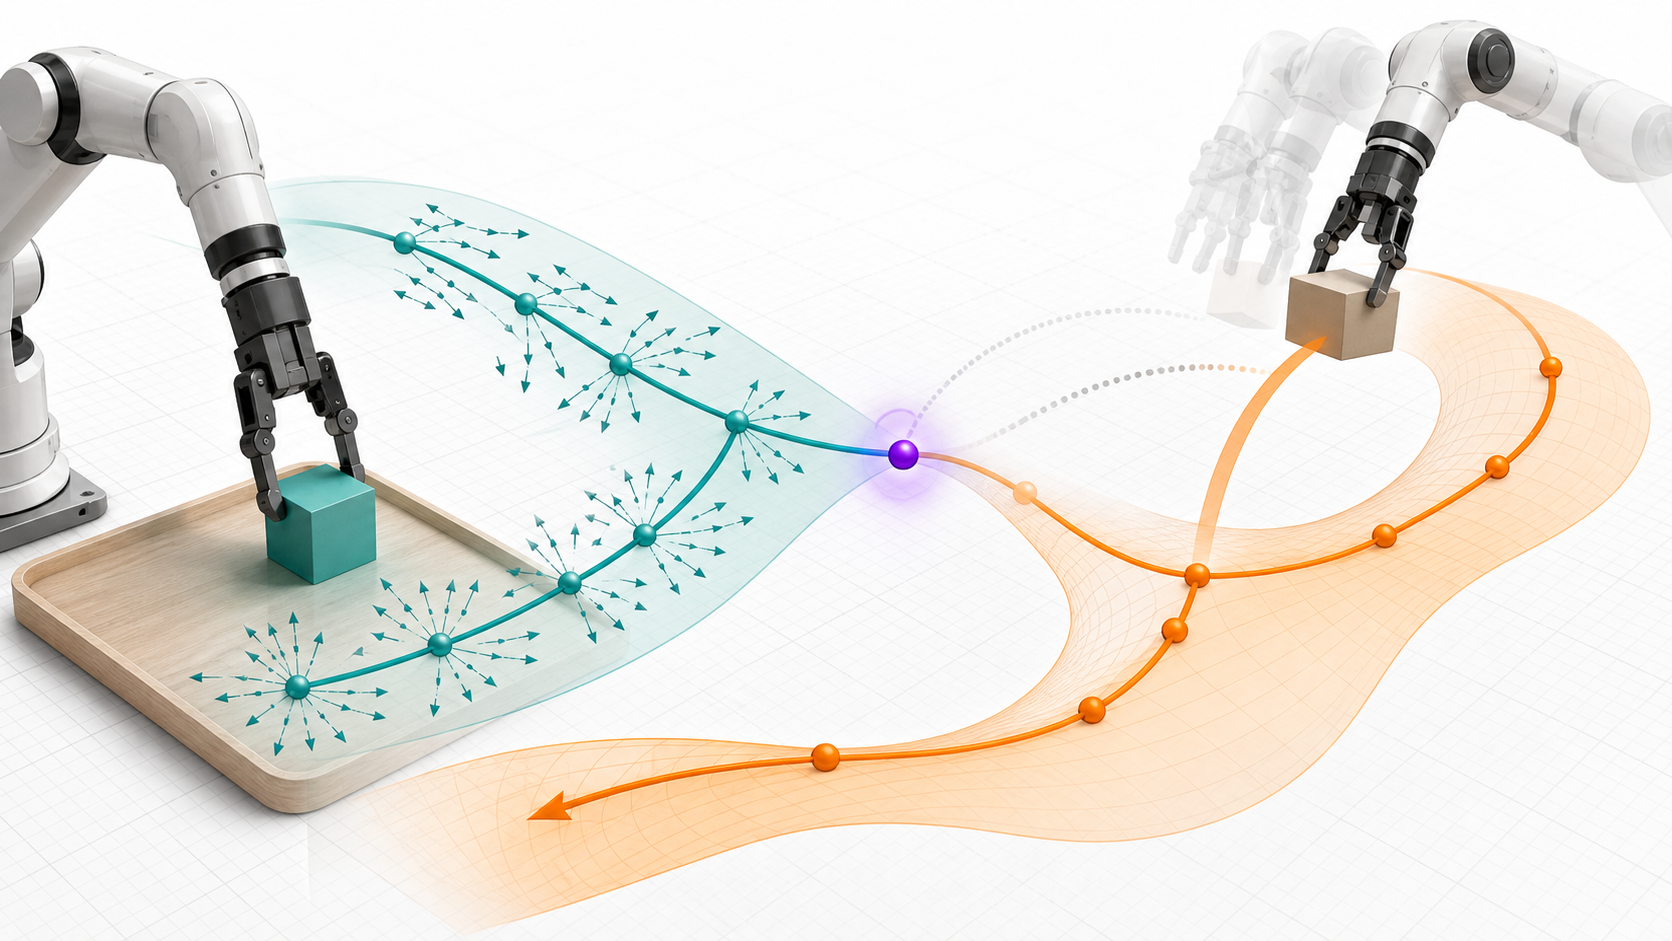
\includegraphics[width=0.96\textwidth]{figures/duet_teaser.png}
\caption{DUET aligns two action geometries for recoverable robot control. Relative actions define a local tangent field around the demonstrated trajectory, while stateless absolute waypoints provide a global state-manifold anchor. When a perturbation moves the robot away from the nominal trajectory, tangent-projection disagreement increases and the policy shifts toward manifold-projection recovery.}
\label{fig:teaser}
\end{figure*}

\section{INTRODUCTION}

Generalist robot policies increasingly use large vision-language models (VLMs) to map images and language instructions to action chunks \cite{rt2,openvla,starvla}. A central design choice in these policies is how actions are represented. We view this choice geometrically, as illustrated in Fig.~\ref{fig:teaser}. Relative controls, such as delta end-effector commands or delta operational-space-control (OSC) actions, parameterize motion as a local vector field around the robot's current configuration. Near the demonstration support, this vector field is smooth, controller-friendly, and tolerant to small pose discrepancies. Away from that support, however, it may remain locally plausible while pointing along the wrong global trajectory. The policy can therefore follow a tangent direction that is well-formed in action space but no longer aligned with the demonstrated task manifold.

Absolute waypoint policies occupy the complementary side of this geometry. By predicting a future end-effector pose directly, they place probability mass on a global state-space trajectory manifold. If the current robot state is perturbed, the difference between a predicted absolute waypoint and the live pose can be interpreted as a projection direction back toward the demonstrated manifold. Yet absolute control is brittle as a primary action representation: it is sensitive to calibration, state-estimation noise, and embodiment-specific coordinate conventions. Thus, relative actions are strong local charts but weak global anchors, while absolute waypoints are strong global anchors but weak default controllers.

DUET is motivated by this dual-manifold view. Instead of choosing one representation, we train a single VLA policy with two action branches: a relative branch that learns a local tangent field for nominal execution and an absolute branch that predicts state-manifold projection targets for global recovery. The key requirement is that the absolute branch must not observe the current robot state. If it does, it can learn the shortcut ``absolute waypoint = current state + delta,'' which collapses the global waypoint branch into another local controller and destroys recovery under OOD states. DUET enforces a stateless absolute branch while still allowing the relative branch to use the current state through both a numerical state encoder and, optionally, a state text segment appended to the VLM prompt.

At inference time, the two branches define a self-contained manifold-consistency signal. The absolute waypoint is converted into a correction command by comparing it with the live pose. When this projection direction disagrees with the relative tangent action, or when the live pose lies outside the training state bounds, DUET increases the absolute-branch fusion weight. Once the state returns to the demonstrated manifold, control smoothly shifts back to the relative branch. This closed-loop gate is simple, does not require a separate OOD classifier, and exposes telemetry that can be plotted over time.

This draft makes the following contributions:
\begin{itemize}
    \item A dual-manifold VLA formulation that interprets relative delta actions as local tangent vectors and stateless absolute waypoints as global state-manifold anchors.
    \item A training recipe that combines residual vector-quantized (RVQ) condition anchoring, classifier-free guidance (CFG), and visual OOD augmentation with gradient truncation on the tangent-field branch.
    \item A closed-loop inference rule that uses tangent-projection disagreement and state-distribution distance to adaptively fuse relative control with absolute recovery.
    \item An implementation in the StarVLA framework and an ICRA-style experimental plan for LIBERO few-shot manipulation and perturbation recovery.
\end{itemize}

\section{RELATED WORK}

\subsection{Vision-Language-Action Policies}
Large VLA models connect visual observations and language instructions to robot actions, often by adapting pretrained VLMs to continuous or discrete action prediction \cite{rt2,openvla,starvla}. RT-2 demonstrated that web-scale vision-language pretraining can transfer semantic knowledge into robotic control \cite{rt2}. OpenVLA provides an open-source VLA model and training recipe \cite{openvla}. StarVLA further emphasizes modular backbones, data loaders, action heads, and deployment interfaces \cite{starvla}. DUET follows this modular view but focuses on a different axis: preserving two action geometries inside one policy and using their disagreement as a recovery signal.

\subsection{Continuous Action Generation}
Diffusion and flow-matching policies generate continuous action chunks and have shown strong performance in manipulation \cite{diffusionpolicy,pi0,gr00t}. These approaches can model multi-modal action distributions and avoid the discretization bottleneck of tokenized action spaces. DUET uses flow-matching action heads for both the relative tangent field and the absolute waypoint manifold. The absolute branch additionally uses classifier-free guidance \cite{cfg} so that its conditioning strength can be adjusted online.

\subsection{Discrete Latent Bottlenecks}
Vector quantization learns a discrete latent codebook that can regularize representations and map inputs to a learned manifold \cite{vqvae,rvq}. DUET uses a residual vector quantizer after learned-query pooling of VLM features. We interpret the codebooks as a discrete atlas over demonstrated visual-language conditions: each quantized token sequence selects a local chart from which the stateless absolute branch predicts a waypoint on the state manifold. The residual norm provides an auxiliary OOD score. In this draft, RVQ is used not for compression but as a condition anchor for recovery-oriented absolute prediction.

\subsection{Robustness and Recovery in Robot Learning}
Robot imitation policies are known to suffer from covariate shift: small errors move the agent into states that are underrepresented in demonstrations. Interactive data aggregation and corrective demonstrations address this by changing the data collection process \cite{dagger}. DUET instead exploits labels already present in datasets such as LIBERO \cite{libero}: relative actions and future absolute end-effector states. The method aims to recover from moderate state perturbations by detecting when the learned local tangent field no longer agrees with a global state-manifold projection.

\section{METHOD}

\subsection{Problem Setup}
At time $t$, the robot observes multi-view images $o_t$, a language instruction $l$, and a current proprioceptive state $s_t$. The policy predicts an action chunk of horizon $K=8$. We use two target representations:
\begin{align}
    \Delta a_{t:t+K-1} &\in \mathbb{R}^{K \times 7}, \\
    W_{t+1:t+K} &\in \mathbb{R}^{K \times 7},
\end{align}
where $\Delta a$ denotes relative OSC commands and $W$ denotes future absolute end-effector waypoints with dimensions $[x,y,z,r,p,y,g]$. The gripper channel in $W$ is treated as an absolute gripper state during training, but the deployed gripper command is taken from the relative branch.

\subsection{Two Action Manifolds}
Let $\mathcal{M}$ denote the demonstrated end-effector state manifold induced by successful task trajectories, and let $T\mathcal{M}$ denote its local tangent bundle. A relative action policy learns a vector field
\begin{equation}
    f_{\mathrm{rel}}(o_t,l,s_t) \in T_{s_t}\mathcal{M},
\end{equation}
which is most reliable when $s_t$ lies near the support of demonstrations. This representation is locally expressive: it specifies how to move from the current chart, but it does not by itself encode where the global trajectory manifold should be.

An absolute waypoint policy instead predicts a future coordinate on the state manifold,
\begin{equation}
    f_{\mathrm{abs}}(o_t,l) = \hat{W}_{t+1:t+K} \in \mathcal{M}^{K}.
\end{equation}
The branch is intentionally stateless with respect to $s_t$, so its prediction is a visual-language-conditioned manifold anchor rather than a current-state-relative displacement. When the robot is perturbed off manifold, the vector from the live pose to this absolute waypoint becomes an empirical projection direction back toward $\mathcal{M}$.

DUET aligns these two geometries online. The relative branch supplies a tangent-following command; the absolute branch supplies a manifold-projection command. Their disagreement estimates whether the local tangent field still agrees with the global demonstrated manifold. Low disagreement indicates that local execution is consistent with the task manifold, while high disagreement signals that a projection-dominated recovery action should take over.

\subsection{Dual-Branch Architecture}
DUET uses a shared Qwen-VL backbone to encode images and instruction tokens. The relative branch attends to the full VLM hidden sequence and receives the normalized current state through a numerical state encoder. The absolute branch receives only RVQ-anchored condition tokens produced from state-free VLM features.

\begin{figure*}[t]
\centering
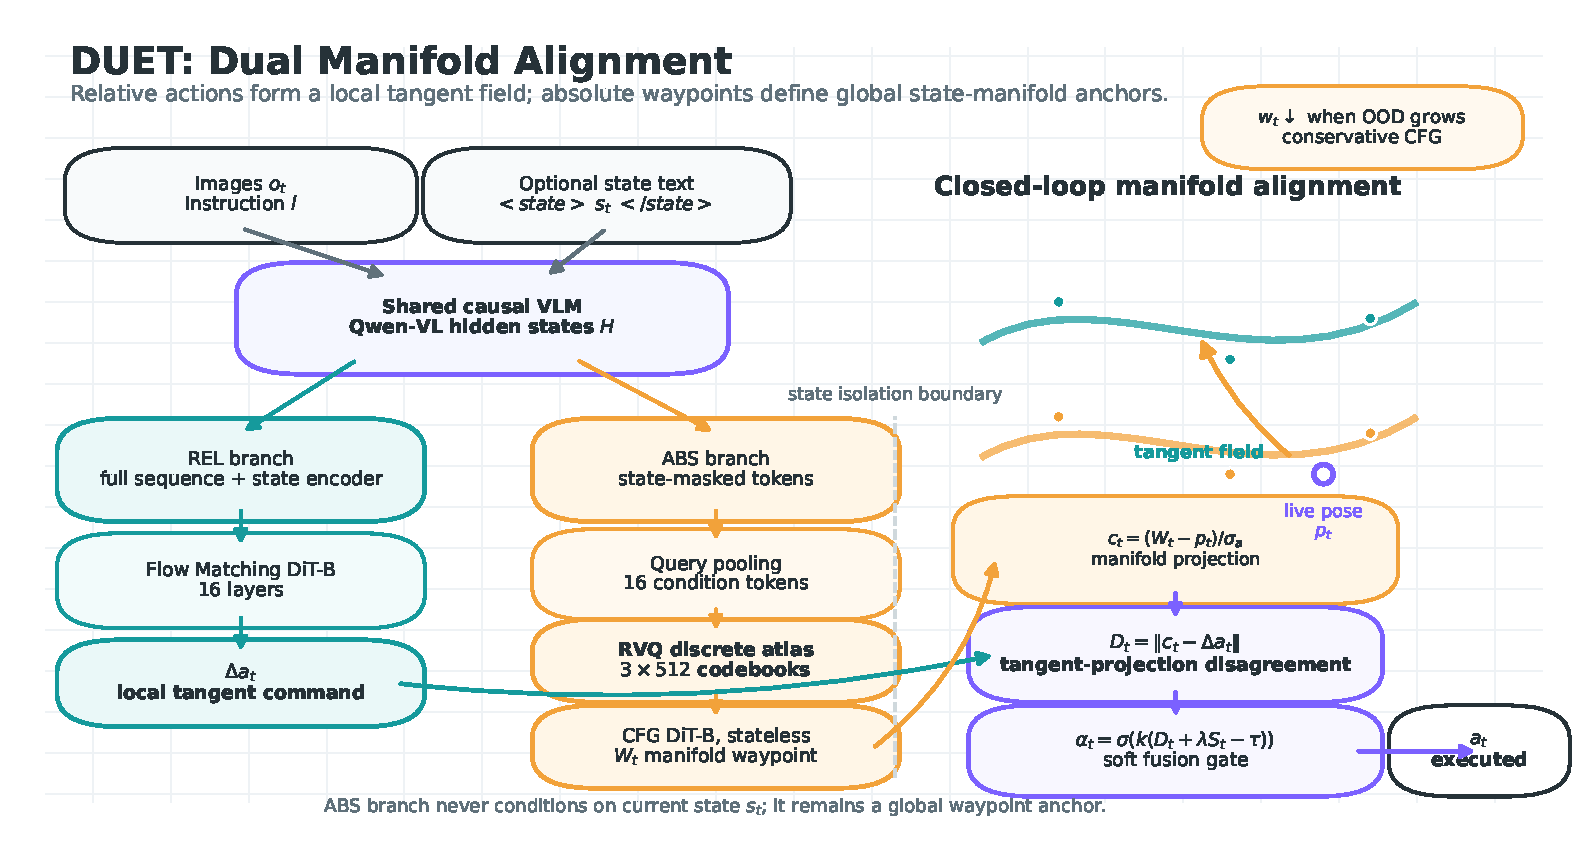
\includegraphics[width=0.98\textwidth]{figures/duet_architecture.pdf}
\caption{Core DUET architecture. A shared causal VLM feeds two action geometries: the relative branch learns a state-aware tangent command, while the absolute branch is state-isolated and predicts a global waypoint through RVQ atlas anchoring and CFG flow matching. At deployment, tangent-projection disagreement and state distance produce a soft fusion gate.}
\label{fig:architecture}
\end{figure*}

The relative branch is intended to be the primary controller under nominal conditions. It learns a smooth local vector field on the action tangent space using a 16-layer DiT-B flow-matching action head with action dimension $7$ and horizon $8$. The absolute branch predicts a state-manifold projection target using a smaller 8-layer DiT-B flow-matching head with state dimension zero. Its output is clamped in normalized space to $[-1,1]$, matching the min-max normalized absolute-state labels.

\subsection{Stateless Absolute Branch}
The central design invariant is:
\begin{quote}
\emph{The absolute branch must not condition on the current robot state $s_t$.}
\end{quote}
DUET supports two state pathways. First, $s_t$ enters the relative branch through a continuous state encoder. Second, when enabled, normalized $s_t$ is formatted as a text segment and appended to the end of the VLM prompt. Because the VLM is causal, earlier token representations do not attend to this final state segment. The absolute branch then constructs a key-padding mask that excludes the state marker, every token after it, and padding positions from RVQ pooling. Thus the relative branch can exploit state-aware VLM features, while the absolute branch remains stateless.

\subsection{RVQ Condition Anchoring}
Let $H \in \mathbb{R}^{B \times L \times d_h}$ be the final VLM hidden sequence after masking out state-contaminated positions for the absolute branch. A learned-query pooling module maps $H$ to $N=16$ latent condition tokens:
\begin{equation}
    Z_e = \mathrm{Pool}(H) \in \mathbb{R}^{B \times N \times d_c}.
\end{equation}
DUET applies residual vector quantization with $M=3$ quantizers:
\begin{align}
    R_0 &= Z_e, \\
    Q_m &= \mathrm{VQ}_m(R_{m-1}), \\
    R_m &= R_{m-1} - Q_m, \\
    Z_q &= Z_e + \left(\sum_{m=1}^{M} Q_m - Z_e\right)_{\mathrm{sg}},
\end{align}
where $\mathrm{sg}$ denotes stop-gradient. The commitment loss is
\begin{equation}
    \mathcal{L}_{\mathrm{vq}} =
    \beta \left\| Z_e - \mathrm{sg}\left(\sum_{m=1}^{M}Q_m\right) \right\|_2^2.
\end{equation}
The final residual norm $\|R_M\|$ is recorded as an auxiliary OOD score. Intuitively, the quantizer maps arbitrary visual-language conditions to nearby codebook combinations, giving the absolute branch a discrete atlas over demonstrated conditions. The waypoint head then predicts from an anchored chart rather than from an unconstrained continuous condition vector.

\subsection{Classifier-Free Absolute Waypoint Head}
During training, the absolute head randomly replaces the quantized condition tokens with learnable null tokens with probability $p_{\mathrm{drop}}=0.15$. At inference time, its flow velocity is computed as
\begin{equation}
    v = v_{\mathrm{uncond}} + w\left(v_{\mathrm{cond}} - v_{\mathrm{uncond}}\right),
\end{equation}
where $w$ is the classifier-free guidance scale. DUET adapts $w$ online using the previous OOD estimate, allowing the absolute branch to move toward a more conservative unconditional state-manifold prior when the robot is strongly OOD.

\section{TRAINING OBJECTIVE}

Each LIBERO training sample provides the relative action chunk and a sequence of current plus future states. We use the dataset action as the relative label and future states $s_{t+1:t+K}$ as absolute waypoint labels after selecting dimensions $[0,1,2,3,4,5,7]$ and min-max normalizing them to $[-1,1]$.

The total loss is
\begin{equation}
\begin{split}
    \mathcal{L} ={}&
    \lambda_{\mathrm{rel}}\mathcal{L}_{\mathrm{rel}}
    + \lambda_{\mathrm{abs}}\mathcal{L}_{\mathrm{abs}}
    + \lambda_{\mathrm{vq}}\mathcal{L}_{\mathrm{vq}} \\
    &+ \lambda_{\mathrm{gate}}\mathcal{L}_{\mathrm{gate}},
\end{split}
\label{eq:training_loss}
\end{equation}
where $\mathcal{L}_{\mathrm{gate}}$ is optional. The default implementation uses equal weights for the relative, absolute, and VQ terms. Both action losses are flow-matching objectives.

\subsection{OOD Augmentation with Relative Gradient Truncation}
For each batch, DUET applies visual perturbations to a subset of samples with probability $p_{\mathrm{aug}}=0.3$. Perturbations include image noise, brightness/contrast/color jitter, and random crop-resize. The absolute branch and RVQ adapter train on both clean and augmented samples, so the manifold anchor remains stable under degraded observations. The relative tangent-field branch computes loss only on clean samples:
\begin{equation}
    \mathcal{L}_{\mathrm{rel}} =
    \frac{1}{|\mathcal{B}_{\mathrm{clean}}|}
    \sum_{i \in \mathcal{B}_{\mathrm{clean}}}
    \ell_{\mathrm{FM}}(\hat{\Delta a}^{(i)}, \Delta a^{(i)}).
\end{equation}
This preserves the relative branch's sensitivity to OOD observations. If both branches were trained to adapt to the same perturbations, their tangent-projection disagreement would become less informative at test time.

\subsection{Optional Learned Gate}
DUET includes an optional second-stage gate. A small MLP receives detached VLM pooled features concatenated with the current state. During training, states are perturbed with Gaussian noise and the gate is supervised with a binary label indicating whether the state was perturbed. At deployment, the gate score can be averaged with the heuristic OOD score.

\section{CLOSED-LOOP MANIFOLD ALIGNMENT}

The policy server returns both unnormalized action representations: a relative chunk $\Delta a_{t:t+K-1}$ and an absolute waypoint chunk $W_{t+1:t+K}$. At each environment step, the client compares the live pose $p_t$ with the current absolute waypoint and converts the difference into an action-space projection command:
\begin{equation}
    c_t = \mathrm{clip}\left(\frac{W_t - p_t}{\sigma_a}, -1, 1\right),
\end{equation}
where $\sigma_a$ contains the position and rotation action scales. In implementation, rotation correction is computed using the geodesic relative rotation rather than an element-wise axis-angle difference.

The tangent-projection disagreement is
\begin{equation}
    D_t = \frac{\left\|c_t^{1:6} -
    \mathrm{clip}(\Delta a_t^{1:6}, -1, 1)\right\|_2}{\sqrt{6}}.
\end{equation}
This quantity is an empirical estimate of manifold inconsistency: it is small when the local tangent vector points in the same direction as the global projection command, and large when local control no longer agrees with the state-manifold anchor. The state-distribution distance measures normalized violation of the training state min-max bounds:
\begin{equation}
    S_t =
    \mathrm{mean}\left[
    \frac{\max(s_{\min} - p_t, 0)}{s_{\max}-s_{\min}}
    +
    \frac{\max(p_t - s_{\max}, 0)}{s_{\max}-s_{\min}}
    \right].
\end{equation}
The OOD score and adaptive fusion weight are
\begin{align}
    q_t &= D_t + \lambda S_t, \\
    \alpha_t &= \sigma(k(q_t-\tau)).
\end{align}
The final action softly transitions between tangent following and manifold projection:
\begin{equation}
    a_t^{1:6} =
    (1-\alpha_t)\Delta a_t^{1:6} + \alpha_t c_t^{1:6},
\end{equation}
with the gripper command copied from the relative branch. When requesting a new action chunk, the client schedules the CFG scale as
\begin{equation}
    w_t = w_{\max} - (w_{\max}-w_{\min})\alpha_{t-1}.
\end{equation}

\begin{figure}[t]
\centering
\fbox{\begin{minipage}{0.94\linewidth}
\small
\textbf{TODO: Insert gate response plot.}

Expected curves: injected perturbation interval, disagreement $D_t$, state distance $S_t$, fusion weight $\alpha_t$, and CFG scale $w_t$ over time.
\end{minipage}}
\caption{Planned closed-loop telemetry visualization for perturbation recovery experiments.}
\label{fig:telemetry}
\end{figure}

\section{EXPERIMENTS}

\subsection{Benchmark and Data}
We evaluate on LIBERO \cite{libero}, using the StarVLA LeRobot data pipeline. The dual-label data configuration uses current plus future state indices $0,\ldots,8$, while action labels use the native delta OSC actions. The default draft configuration trains on the \texttt{libero\_10\_hybrid} mixture, with planned extensions to \texttt{libero\_all\_hybrid}. For few-shot experiments, the data loader limits demonstrations per task through \texttt{max\_demos\_per\_task}.

\subsection{Implementation Details}
DUET is implemented as \texttt{QwenGR00THybrid} in StarVLA. The backbone is Qwen-VL with hidden dimension $2048$. The relative branch uses a 16-layer DiT-B flow-matching head. The absolute branch uses an 8-layer DiT-B flow-matching head with $16$ RVQ condition tokens of output dimension $1024$. RVQ uses three residual quantizers with codebook size $512$ and code dimension $256$. Training uses AdamW and the schedule specified in the repository configuration.

\subsection{Perturbation Recovery Protocol}
To test recovery, we inject an action-space perturbation for a fixed interval during rollout. The evaluation script supports perturbation start step, duration, and magnitude. We record success, action traces, dual-branch disagreement, state-distance score, fusion weight, and CFG scale for each episode.

\subsection{Main Results}

\begin{table}[t]
\caption{LIBERO success rates. All quantitative entries are TODO placeholders and must be filled after running evaluation.}
\label{tab:main_results}
\centering
\resizebox{\columnwidth}{!}{%
\begin{tabular}{lccc}
\toprule
Method & Demos/task & Clean SR & Perturbed SR \\
\midrule
Relative-only VLA & TODO & TODO & TODO \\
Absolute-only waypoint & TODO & TODO & TODO \\
Fixed fusion, $\alpha=0.5$ & TODO & TODO & TODO \\
DUET adaptive & TODO & TODO & TODO \\
DUET + learned gate & TODO & TODO & TODO \\
\bottomrule
\end{tabular}
}
\end{table}

Table~\ref{tab:main_results} will report the main clean and perturbation recovery success rates. The expected analysis is that relative-only control should be competitive on clean rollouts but less robust under perturbation, while DUET should improve recovery by increasing the manifold-projection weight only when needed.

\subsection{Ablations}

\begin{table}[t]
\caption{Planned ablations. TODO entries should be filled with success rate, recovery rate, and telemetry statistics.}
\label{tab:ablations}
\centering
\begin{tabular}{lcc}
\toprule
Ablation & Clean SR & Perturbed SR \\
\midrule
DUET full & TODO & TODO \\
No RVQ anchoring & TODO & TODO \\
No CFG adaptation & TODO & TODO \\
No relative gradient truncation & TODO & TODO \\
State-to-VLM disabled & TODO & TODO \\
Fixed $\alpha=0$ & TODO & TODO \\
Fixed $\alpha=1$ & TODO & TODO \\
\bottomrule
\end{tabular}
\end{table}

The ablations in Table~\ref{tab:ablations} isolate the contribution of condition anchoring, guidance adaptation, branch specialization, state prompt injection, and adaptive fusion. Additional metrics should include mean maximum displacement after perturbation, mean recovery time, and area under the $\alpha_t$ curve.

\section{LIMITATIONS}

DUET assumes access to absolute state labels aligned with the relative action chunks. This is natural in LIBERO and many robot logs, but may require additional calibration or state estimation on real hardware. The closed-loop gate currently uses simple min-max state statistics as a coarse proxy for distance to the demonstrated state manifold, which may be insufficient for highly multi-modal workspaces. The absolute branch is deliberately stateless; while this supports recovery, it may reduce waypoint accuracy in tasks where the current robot state contains task-relevant information not recoverable from images. Finally, all quantitative claims in this draft remain pending until the planned LIBERO and perturbation experiments are completed.

\section{CONCLUSION}

We presented DUET, a dual-branch VLA policy that aligns a local relative-action tangent field with a stateless absolute-waypoint manifold. By enforcing state isolation in the absolute branch, anchoring its condition with RVQ, and using online tangent-projection disagreement to gate fusion and guidance, DUET turns two complementary action geometries into a closed-loop recovery mechanism. The implementation is integrated into StarVLA and is ready for LIBERO few-shot and perturbation recovery evaluation.

\section*{ACKNOWLEDGMENT}

TODO: Add acknowledgments, funding, compute resources, and any required dataset or codebase acknowledgments after the author list is finalized.

\bibliographystyle{IEEEtran}
\bibliography{references}

\end{document}
